\section{Motivation} \label{sec:motivation}
%\vspace{-5pt}
%
In this section, we first present the system model of TPCs in Sec.~\ref{sec:motiModel}. 
Then, we use an image sensing example to show the needs for hardware support in Sec.~\ref{sec:motiHW} and challenges of recovering a TPC with multiple peripherals in Sec.~\ref{sec:motiSW}. 

%
\begin{figure}[t]
    \centering
    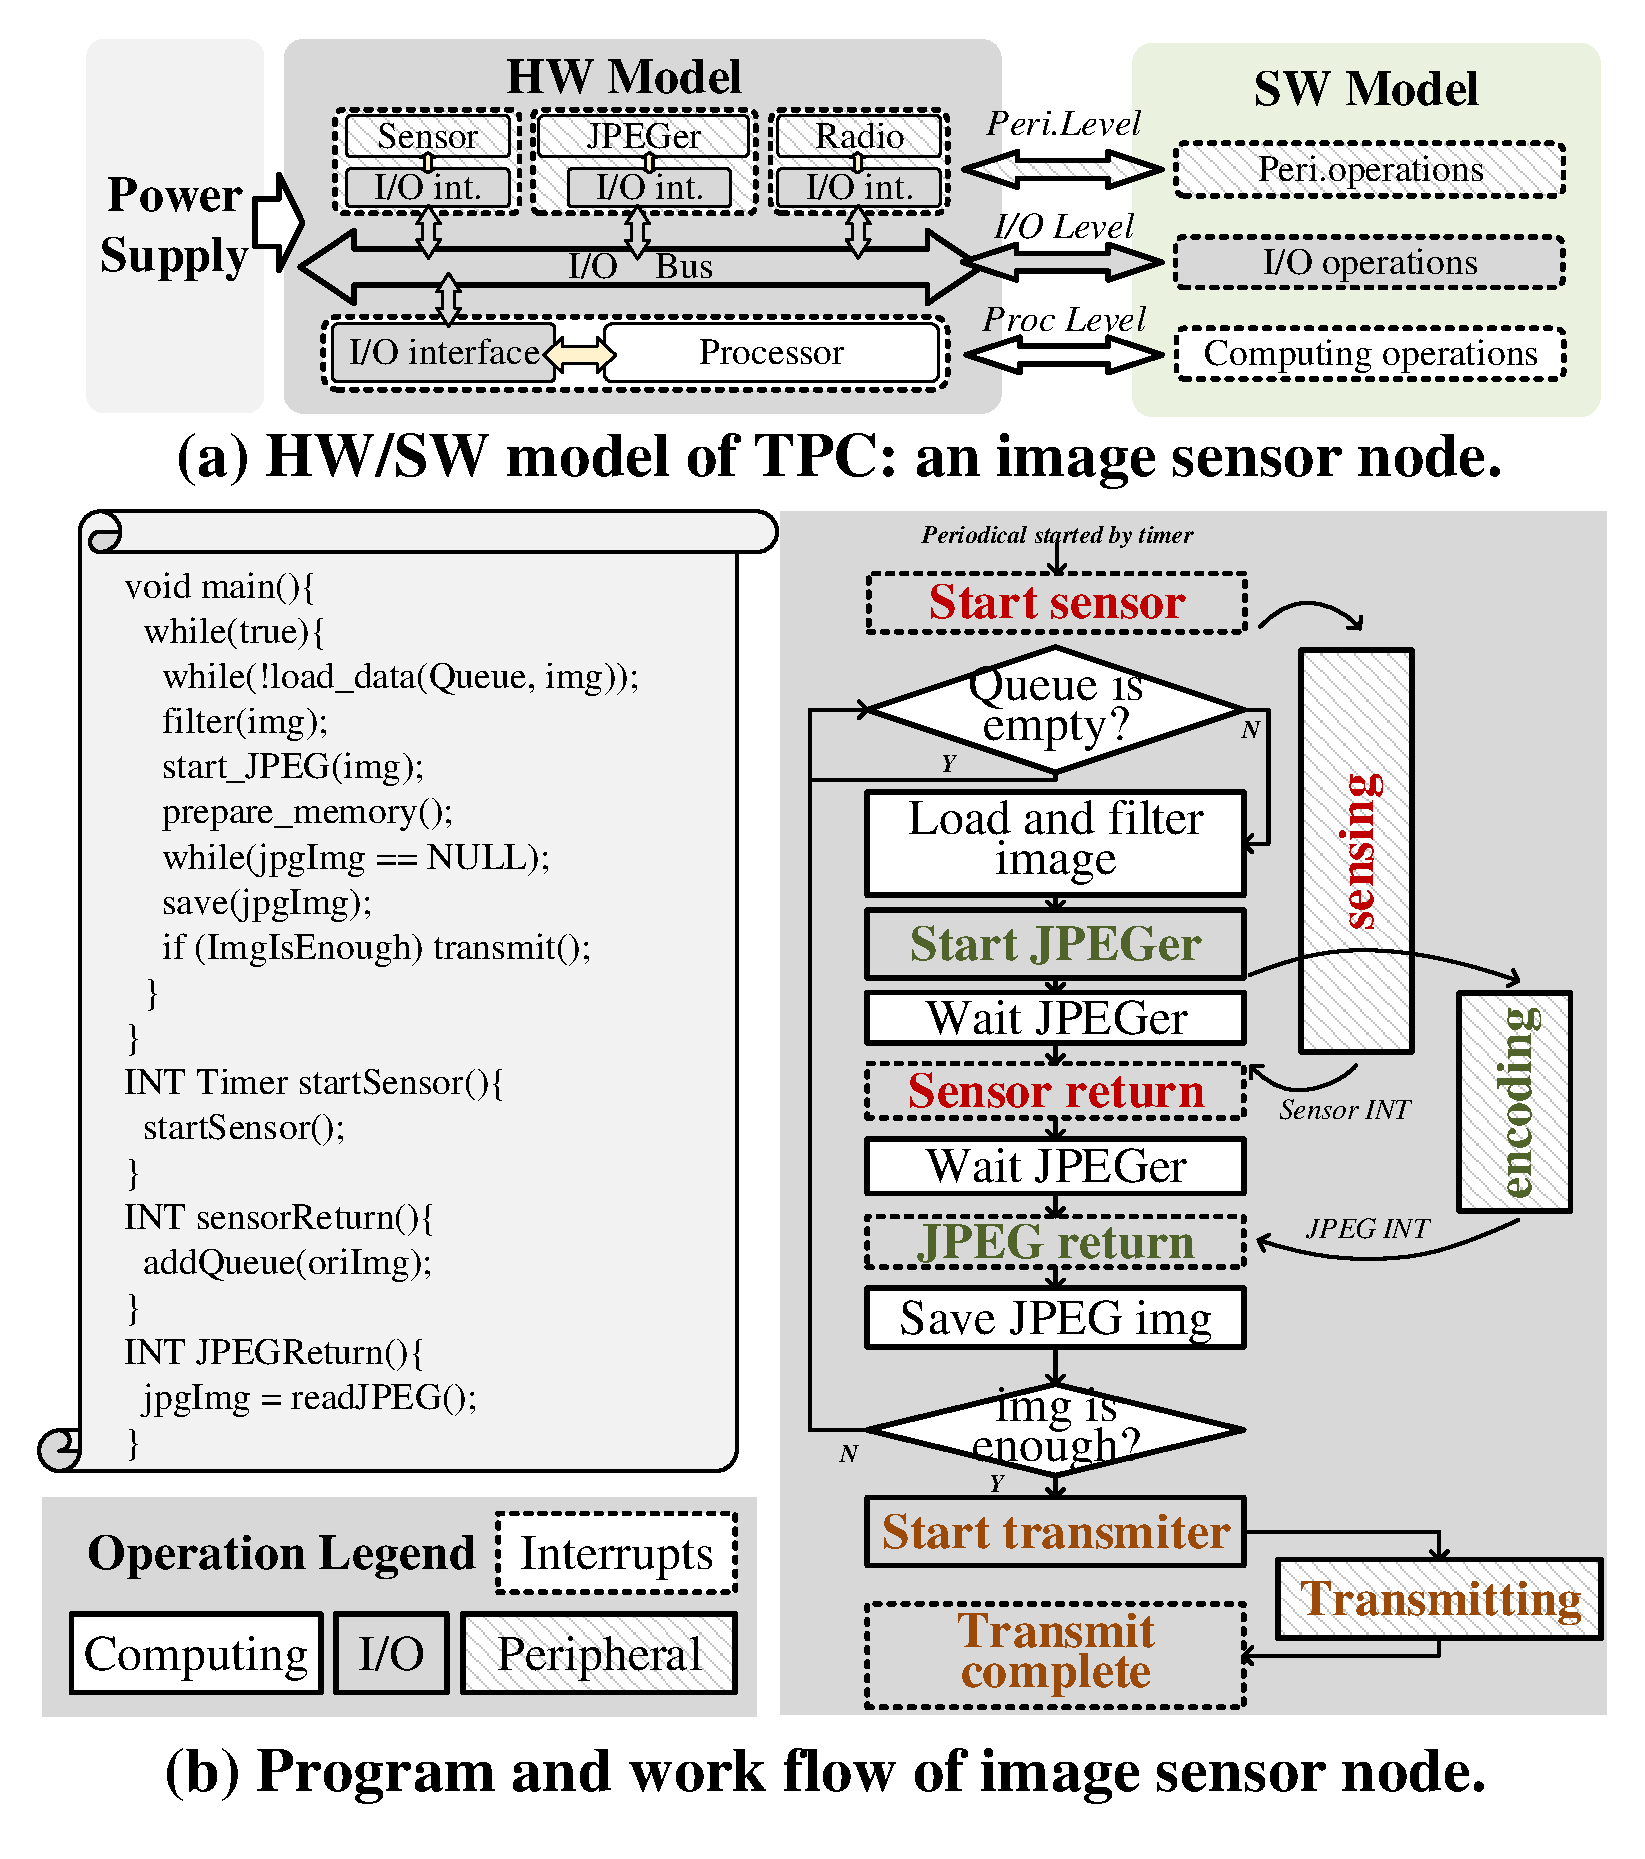
\includegraphics[width=0.47\textwidth]{Fig1_TPCModel.pdf}
    \vspace{-10pt}
    \caption{An image sensing example used to present the HW/SW model of TPC system.}
    \vspace{-5pt}
    \label{fig:TPCmodel}
\end{figure}

%\vspace{-5pt}
\subsection{TPC System Model} \label{sec:motiModel}
\vspace{-5pt}
%
% Problem model and the requirements
Fig.~\ref{fig:TPCmodel} (a) uses an image sensing example to show the HW/SW models of a multi-device TPC system.
The devices contain a processor and multiple peripherals.
The sensor node utilizes a processor to execute \emph{computing operations} and controls peripherals.
Peripherals, such as sensors and wireless transceiver, are used to perform specific \emph{peripheral operations} in parallel. 
These peripherals can be divided into three categories.
The input-type collects the environmental information, such as the image sensor.
The output-type transmits data to other systems, such as the wireless transceiver.
The compute-type accelerates computing intensive tasks, such as a JPEG encoder.
Processor and the peripherals are mounted to an I/O bus via on-chip I/O interfaces, where I/O operations are executed.
With \emph{I/O operations}, the processor initializes, configures and accesses the peripherals by reading and writing their embedded memory. 

Fig.~\ref{fig:TPCmodel} (b) shows the program and the work flow of this image sensor node.
The image sensor is periodically started by a timer to collect and store images in a queue.
In the loop of main function, the system first load and filter an original image from the queue.
Then, the JPEGer is called to encode the image.
Both the sensor and the JPEGer return their results through hardware interrupts.
The processor will finally store the encoded image in memory.
When the stored images reach a threshold, the transceiver send these images to the server.

%\begin{table}[t]
\caption{I/O and peripheral support of existing works.}\label{tab:preWork} %I/O and peripheral recover support of representative existing works
\centering
\Fsize{8}
\renewcommand{\arraystretch}{1.5}
\begin{tabular}{IcIcIcIcIcIcI}
    \Xhline{1.2pt}
    Solution            & HW Model                 & I/O rec.          & peri rec.                     & B/R              & Ref.\\
    \Xhline{1.2pt}
    Mementos        & VP + Flash                 & $\times$        & $\times$                     & >10ms         &~\cite{ransford2012mementos}\\
    \Xhline{1pt}
    Hibernus          & VP + FRAM              & $\times$         & $\times$                     & 5.05ms         &~\cite{balsamo2015hibernus} \\
    \Xhline{1pt}
    QuickRecall     & VP + FRAM              & $\surd$           & $\surd$                      & 168us          &~\cite{jayakumar2014quickrecall}\\
    \Xhline{1pt}
    NVP                 & NVP + VIO                & $\times$        & $\times$                     & 8us             &~\cite{wang20123us}\\
    \Xhline{1pt}
    NVIO               & NVP + NVIO             & $\surd$          & $\times$                     & 8us             &~\cite{li2016hw}\\
    \Xhline{1.2pt}
\end{tabular}
\end{table} 
%
In such a system, the processor can be efficiently recovered with existed techniques. 
However, peripherals will lose their states after power failure, which leads to reliability and efficiency issues. 
Based on the type of peripherals, different faults will occur if the devices are not recovered: 
\textbf{1. Input-type Failure:} When a sensor loses power, the current collection will be crashed and data is lost. 
Even worse, one data lost may jeopardize the integrity of the whole data set in a multi-sensor system.
\textbf{2. Output-type Failure:} When a transceiver loses power, the current transmitting package as well as the data in peripheral buffer will be lost. Although costly software-level re-transmission can be used in some cases, it may not be feasible for resource-constraint energy-harvesting sensors. 
\textbf{3. Compute-type Failure:} When an accelerator loses power, processor cannot receive its returned results and halts all subsequent operations.
It may cause system deadlock when program relies on the returned data.
Therefore, a systematical peripheral recovery mechanism is in desperate needs. 

\begin{figure}[t]
    \centering
    \includegraphics[width=0.48\textwidth]{Fig1_motiNVM}
    \vspace{-15pt}
    \caption{Hardware challenges of multi-device checkpointing. NVP is limited by passive B/R function. Peripherals require efficient reconfigurations and restarts.}
    \vspace{-5pt}
    \label{fig:motiNVM}
\end{figure}

Targeting on the multi-device TPC, two challenges arise.
(a) How to design an efficient and reliable architecture to recover the states of the peripherals in a multi-device system;
(b) How to devise a reliable automatic checkpointing mechanism for a TPC with multiple devices.
The rest of this paper addresses these two challenges.

%\vspace{-5pt}
\subsection{Hardware Needs for Peripheral Recovery} \label{sec:motiHW}
\vspace{-5pt}
%
Fig.~\ref{fig:motiNVM} shows the NVP~\cite{wang20123us} achieving efficient recovery by backing up and restoring (B/R) the processor state, when the voltage detector is triggered by a power failure.
The B/R operation of processor is passively activated by the voltage detector.
However, consistency problems may exist when a power failure occurs during a peripheral operation.
This is because peripherals can only back up their states at certain safe positions.
Therefore, multi-device TPC requires flexible B/R interfaces instead of the passive approach based on voltage detector in existing NVPs.

% peripheral recover problem: restore and restart
Furthermore, an efficient recovery monitor for volatile peripherals besides the NVP is needed.
Fig.~\ref{fig:motiNVM} shows the structure of an image sensor, a typical volatile peripheral.
Its digital part uses registers to store the data and device state, and the analog part collects images from environment.
When the system recovers a peripheral after power failures, not only the digital part should be restored, but also the analog part. 
On the other hand, not all peripherals should be recovered in a multi-device TPC especially those are not used. 
As the number of peripherals increases, the recovery overhead becomes significant. 
Thus, a peripheral status monitoring module is needed to avoid unnecessary peripheral reconfiguration overhead.

Last but not least, once a peripheral device is determined to be restarted after power failure, e.g. the sensing and data transmission task in the image sensor node, a specific start function should be re-executed. 
In existing NVPs, those operations are restarted by rolling the entire system back to where the broken peripheral operations just started. Extra rollback overhead takes place because the program cannot return correctly after executing the start program. If a hardware module can simply re-execute the peripheral start program and return correctly, the peripheral restart can be more efficient.

Therefore, to efficiently and reliably recover multi-device TPCs, the enhanced NVP should support flexible checkpointing, peripheral status monitor as well as the peripheral restart modules, which are all missing in existing NVPs.

%   
\begin{figure}[t]
    \centering
    \includegraphics[width=0.48\textwidth]{Fig1_motiRollback}
    \vspace{-12pt}
    \caption{Challenges using single-device checkpointing strategies in a multi-device system. A distributed and reliable checkpointing framework is needed.}
    \vspace{-5pt}
    \label{fig:motiRollback}
\end{figure}

\subsection{Multi-device Checkpointing Challenges} \label{sec:motiSW}
\vspace{-5pt}
%
Even with the hardware described in Sec.~\ref{sec:motiHW}, it is still nontrivial to recover multi-device system efficiently and reliably. 
Fig.~\ref{fig:motiRollback} shows the recover flows of the image sensor when a power failure occurs.
There are three processes in each figure.
The bottom is processor process, which executes the main program given in Fig.~\ref{fig:TPCmodel}.
The middle is sensor process and the top is JPEGer process. 
These two modules are started by the processor, and return their results via interrupts after completing the sensing and encoding tasks.
When power fails and crashed both of the peripherals, traditional single-device approaches~\cite{ransford2012mementos, balsamo2015hibernus, jayakumar2014quickrecall} roll back the entire system to a homogeneous checkpoint.
If \emph{cp1} is selected, all peripherals can be correctly recovered but nontrivial rollback overhead is introduced for both processor and the JPEGer. 
The processor rolls back for 135ms and the JPEGer has to wait 79ms to restart.
If \emph{cp3} is selected, the rollback overhead is smaller but inconsistency arises. 
The image sensor is not recovered, and the processor receives wrong data.

An ideal multi-device recovery should support different devices to roll back separately with minimum overheads while maintaining system consistency. 
In Fig.~\ref{fig:motiRollback} (b), if the processor is restored to the interrupt position without rollback and the JPEGer is also restarted instantly, the recovery overhead can be reduced by 58.5\%.
However,  \emph{cp3} is still not the correct position because of the inconsistency problem. \emph{cp4} is a more reliable checkpoint located before the interrupt, which prevents the processor from receiving erroneous data.
Therefore, an automatic checkpointing tool supporting individual and reliable recovery of multi-device  TPCs is also needed even with the enhanced hardware. 










